\documentclass[11pt, a4paper]{article}
\usepackage[a4paper, total={6.5 in,9in}]{geometry}
\usepackage[slovene]{babel}
\usepackage[utf8]{inputenc}
\usepackage[T1]{fontenc}
\usepackage{lmodern}
\usepackage{amsmath}
\usepackage{ amssymb }
\usepackage{amsfonts}
\usepackage{amsthm}
\usepackage{comment}
\usepackage{url}
\usepackage{gensymb}
\usepackage{subcaption}
\usepackage[pdftex]{graphicx}
\usepackage[section]{placeins}
\usepackage{mathtools}
\usepackage{float}
\usepackage{epstopdf}
\renewcommand{\vec}[1]{\mathbf{#1}}
\usepackage{hyperref}
\usepackage{wrapfig}
\usepackage{mhchem}
\pagestyle{plain}

\begin{document}

    \begin{center}
    {\LARGE\bfseries 5. Modeli kemijskih reakcij\par}
    \vspace{1cm}
    
    {\Large Domača naloga pri predmetu Modelska analiza I\par}
    \vspace{0.2cm}
    {\normalsize Avtor: Matic Noč \par}
    \vspace{0.2cm}    
    {\normalsize 5.11.2017 \par}    

    
    \end{center}

\section{Uvod}
Naloga obravnava binarne modele kemijskih reakcij, k jih lahko, če poznamo parametre verjetnosti za reakcijo v določeni smeri, opišemo s sistemom navadnih diferencialnih enačb v stilu logističnih enačb, le da tu ni treba srečanja dveh substanc za nastanek novih produktov.
\section{Model binarnih reakcij}
Poglejmo si binarno rekacijo, to je reakcija, kjer interagirata največ dva reagenta:
\begin{equation}
\ce{A + A <=>[\ce{p}][\ce{q}] A + A^*}
\end{equation}
\begin{equation}
\ce{A^* ->[\ce{r}] B + C}
\end{equation}
Vzeli bomo $\frac{q}{p}=1000$, kar pomeni veliko hitrejše nastajanje nastajanje reaktantov v levi smeri , potem pa pagledali kaj se zgodi za različne r. Videli bomo, da zaradi tega $A^*$ zelo hitro razpade v ostale produkte, torej \textbf{ Kar koli $A*$ nastane se zelo hitro spremeni v B in C ali pa nazaj v A in A. Torej se zelo hitro prilagodi v neko stacionarno stanje, kjer toliko $A*$ kot nastane takoj izgine oziroma je zato spreminjanje enako 0 oziroma $\dot{[A*]} = 0$, kar lahko upoštevamo pri reševanju problema in se tako znebimo ene prostostne stopnje}. Opomniti moramo, da se po dolgem času to zgodi tudi z ostalimi substancami - \textbf{ enaka količina kot substance nastane, tudi zreagira in s tem ohranja ravnotežno stanje reakcije.} \newline\newline Vsaka reakcija ima 
parameter verjetnosti za reakcijo. Sistem se obnaša podobno, kot populacijski sistemi; \textbf{več molekul imamo, hitreje bodo nastajali novi, saj je verjetnost za reakcijo večja.} Ker se z vsemi reaktanti dogaja podobno lahko namesto ene reakcije zapišemo sistem za spreminjanje koncentracij, ki ga imenujemo \textit{reaction rate equations}. 
\begin{equation}
\dot{[A]} = -p[A]^2+q[A][A^*],
\end{equation}
\begin{equation}
\dot{[A^*]} = p[A]^2-q[A][A^*]-r[A^*],
\end{equation}
\begin{equation}
\dot{[B]} = \dot{[C]}=r[A^*]
\end{equation}
Enačbe bomo najprej reševali z  numerično integracijo celotnega sistema, nato reševali s aproksimacijo stacionarnega stanja za $[A*]$. Poglejmo si osnovne značilnosti rešitev.\newline
\subsection{Reševanje sistema}
\begin{figure}[H]
\hspace*{-1cm}     
  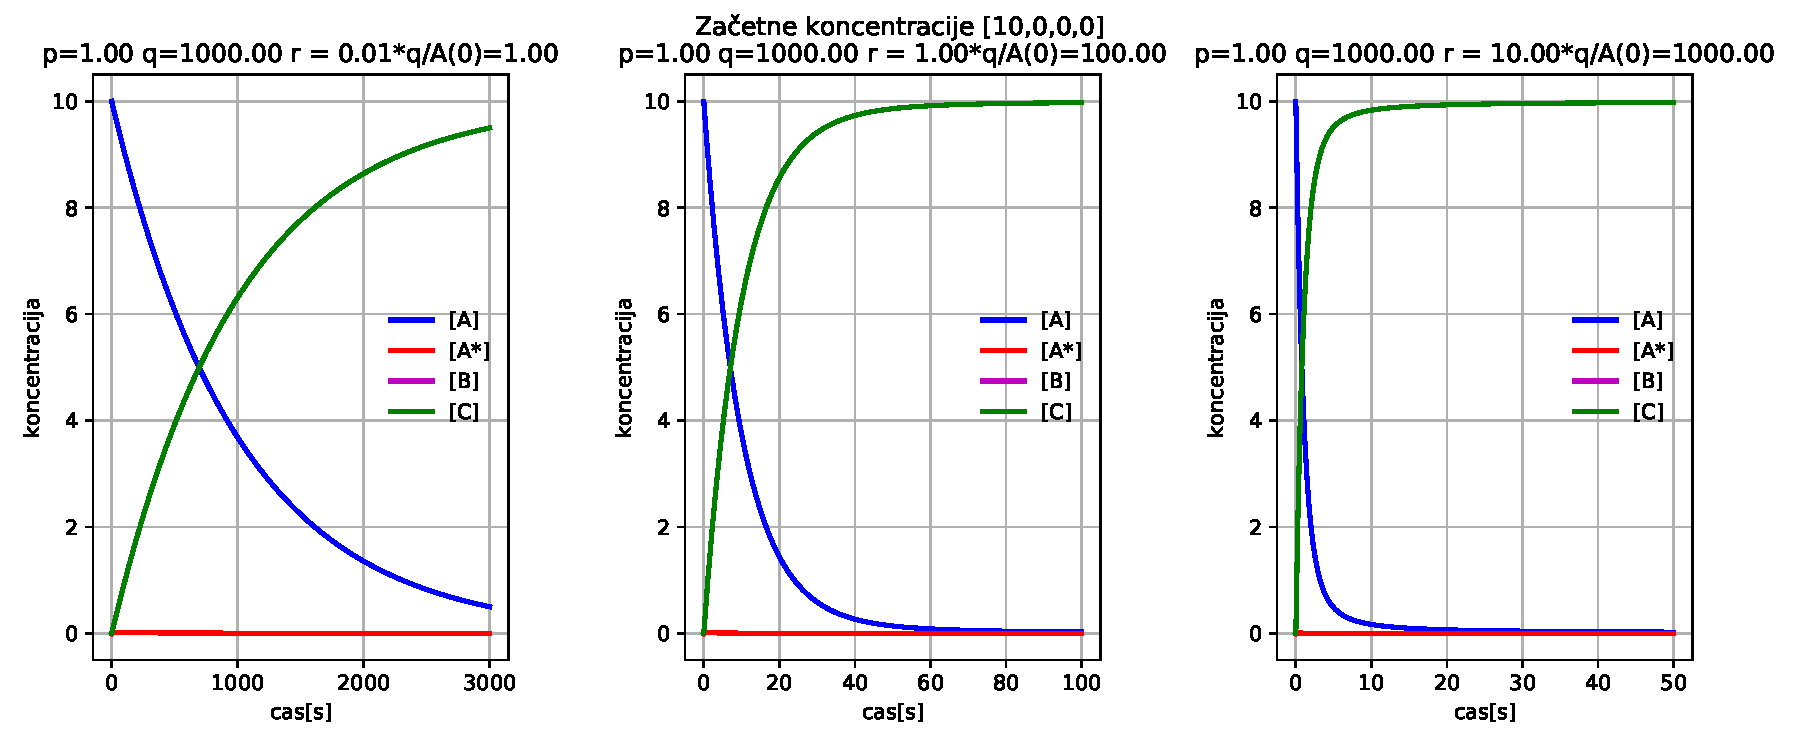
\includegraphics[width=20cm]{prva_osnovni_zacet_pogoji.pdf}
  \caption{Začetne koncentracije [A,A*,B,C] = [10,0,0,0]. Spreminjanje hitrosti reakcije $r$, torej A* v B in C nam pospeši nastajanje končnega elementa B in C (se prekrivata). Vidimo tudi, da je [A*] ob stacionarnem stanju skoraj 0, vendar ne čisto 0.}
\end{figure}

\begin{figure}[H]
\hspace*{-1cm}     
  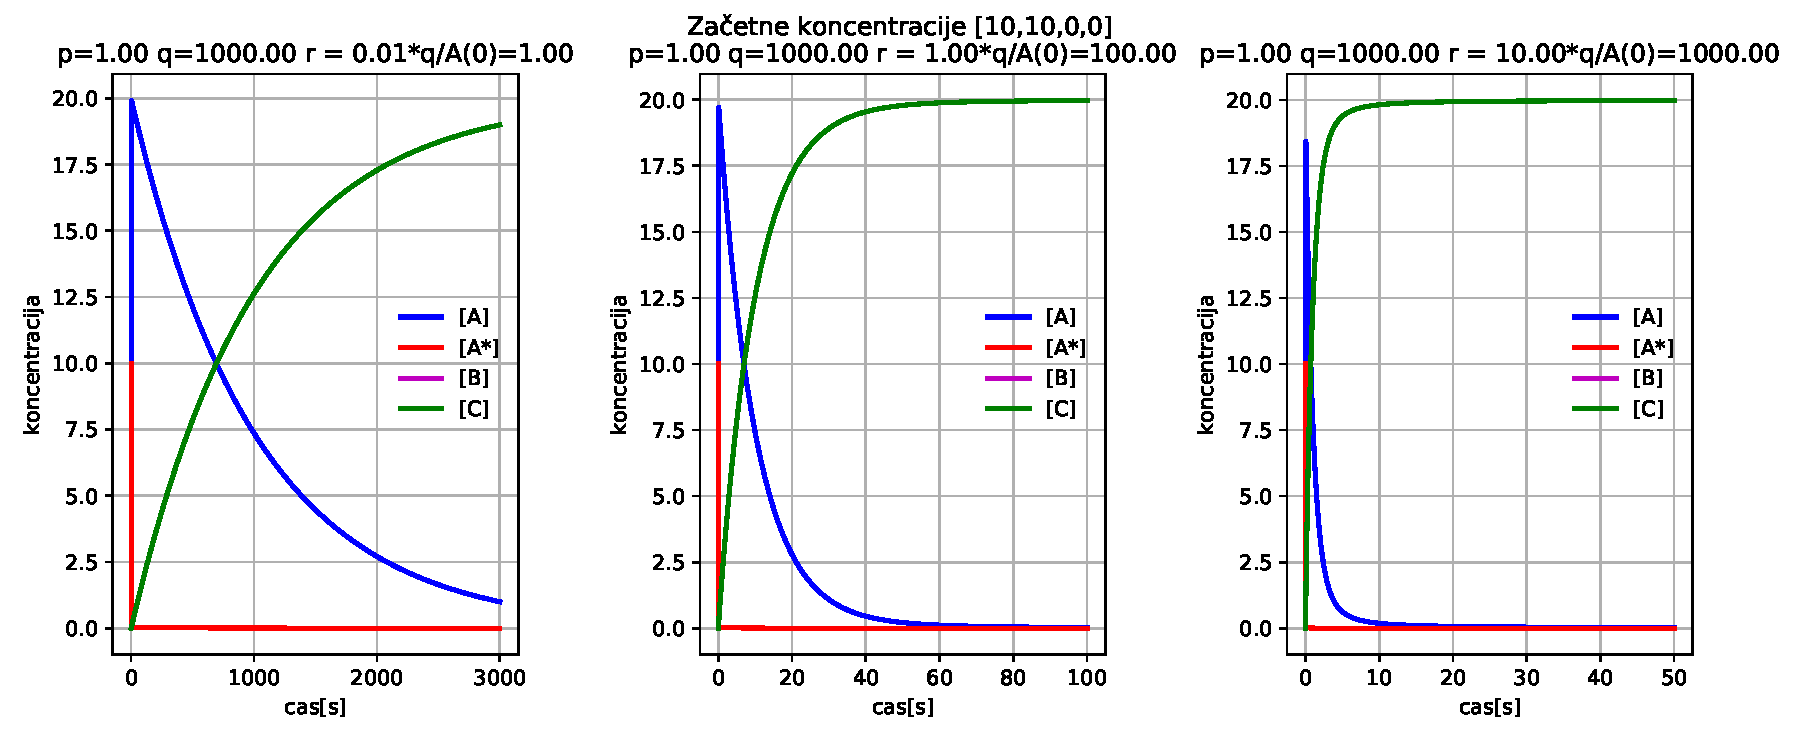
\includegraphics[width=19cm]{prva_drugi_zacet_pogoji.pdf}
  \caption{Začetne koncentracije [A,A*,B,C] = [10,10,0,0]. Tu spremenimo začetno koncentracijo A* in vidimo kako hitro A naraste in A* pade v stacionarno stanje, ko se vsi A*, ki nastanje spremenijo v B in C, katerih koncentraciji sta skoraj enaki koncentraciji A na začetku. Ko [A], [A*] ni več, [B] in [C] ne moreta več nastajati, oziroma se vzpostavi končno stanje, ko kemijskih reagentov ni več za naprejšni potek reakcije.} 
\end{figure}
Poglejmo si kaj se zgodi če hitrost reakcij obrnemo, tako da je $p$ velik in $q$ majhen. Takrat bi vsak A, ki bi nastal, takoj reagiral z A in tako bi nastal nazaj A*.\newline

\begin{figure}[H]
\hspace*{-1cm}     
  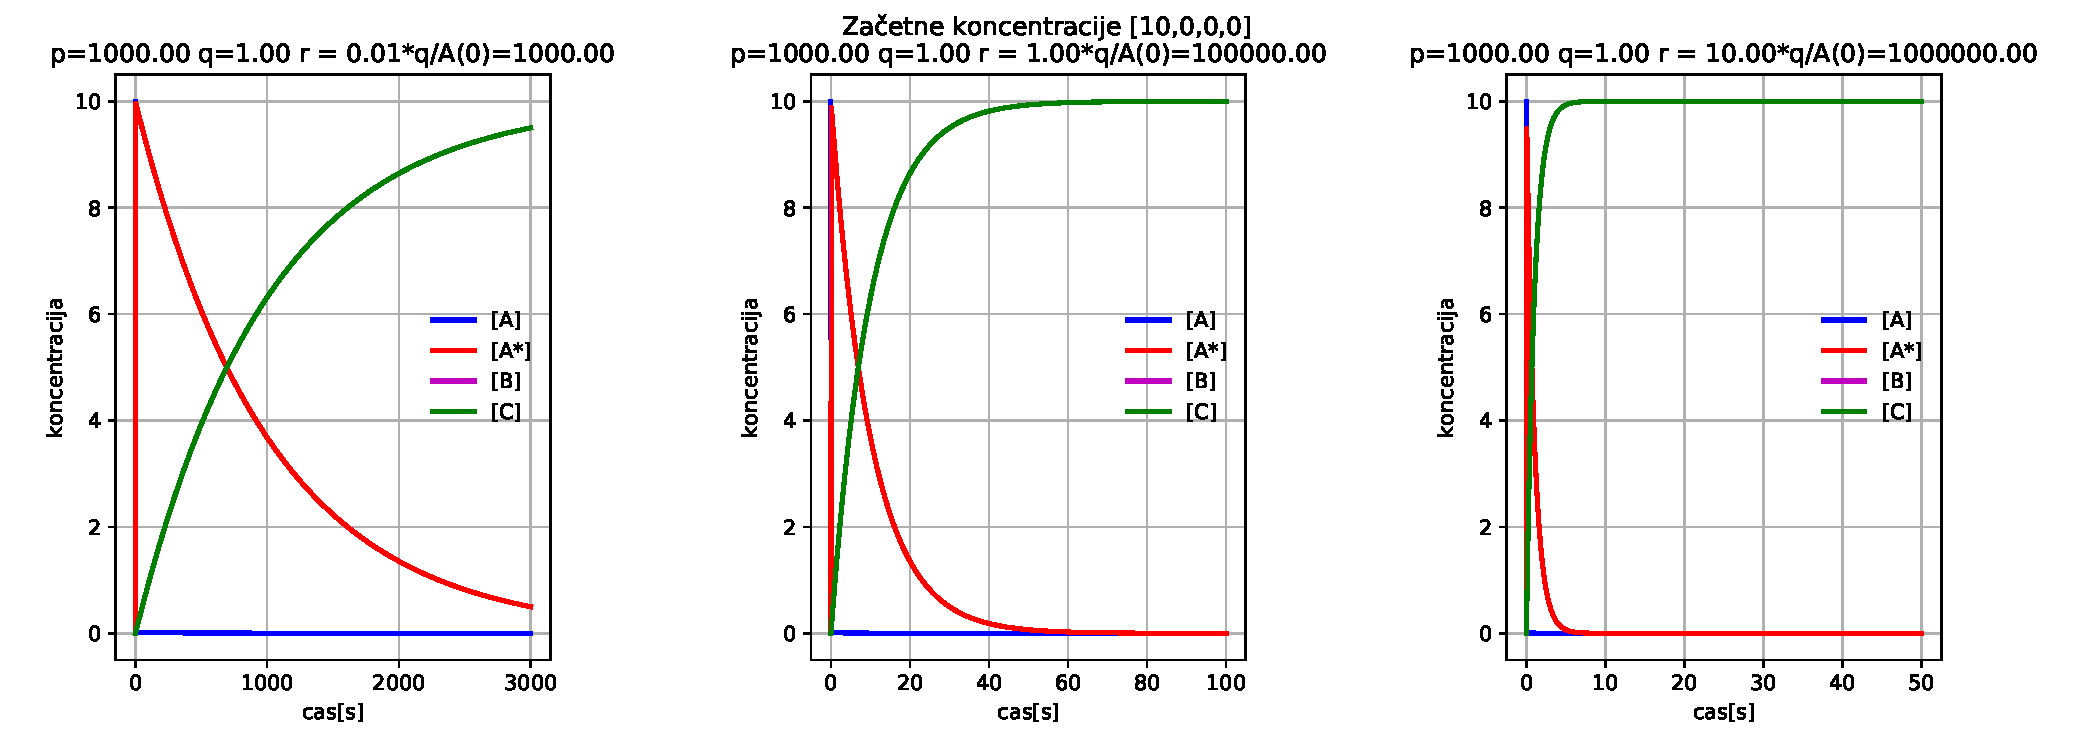
\includegraphics[width=20cm]{prva_obratna_reakcija.pdf}
  \caption{Obratna smer reakcije, ko je $p$ velik in $q$ majhen. Vidimo, A takoj upade, A* naraste in se nato z različnimi hitrostmi spreminja v B in C } 
\end{figure}
\subsection{Stacionarno stanje}
Postavimo sedaj  $\dot{[A*]} = 0$ in dobimo stacionarno stanje za A*:


\begin{equation}
\dot{[A^*]} =0= p[A]^2-q[A][A^*]-r[A^*],
\end{equation}
\begin{equation}
[A^*] = - \frac{p[A]^2}{q[A] + r} 
\end{equation}
V našem primeru, tudi če imamo kaj A, sta q in r velika in zato bo $[A^*] \sim 0$
\begin{figure}[htbp]
\hspace*{-1cm}     
  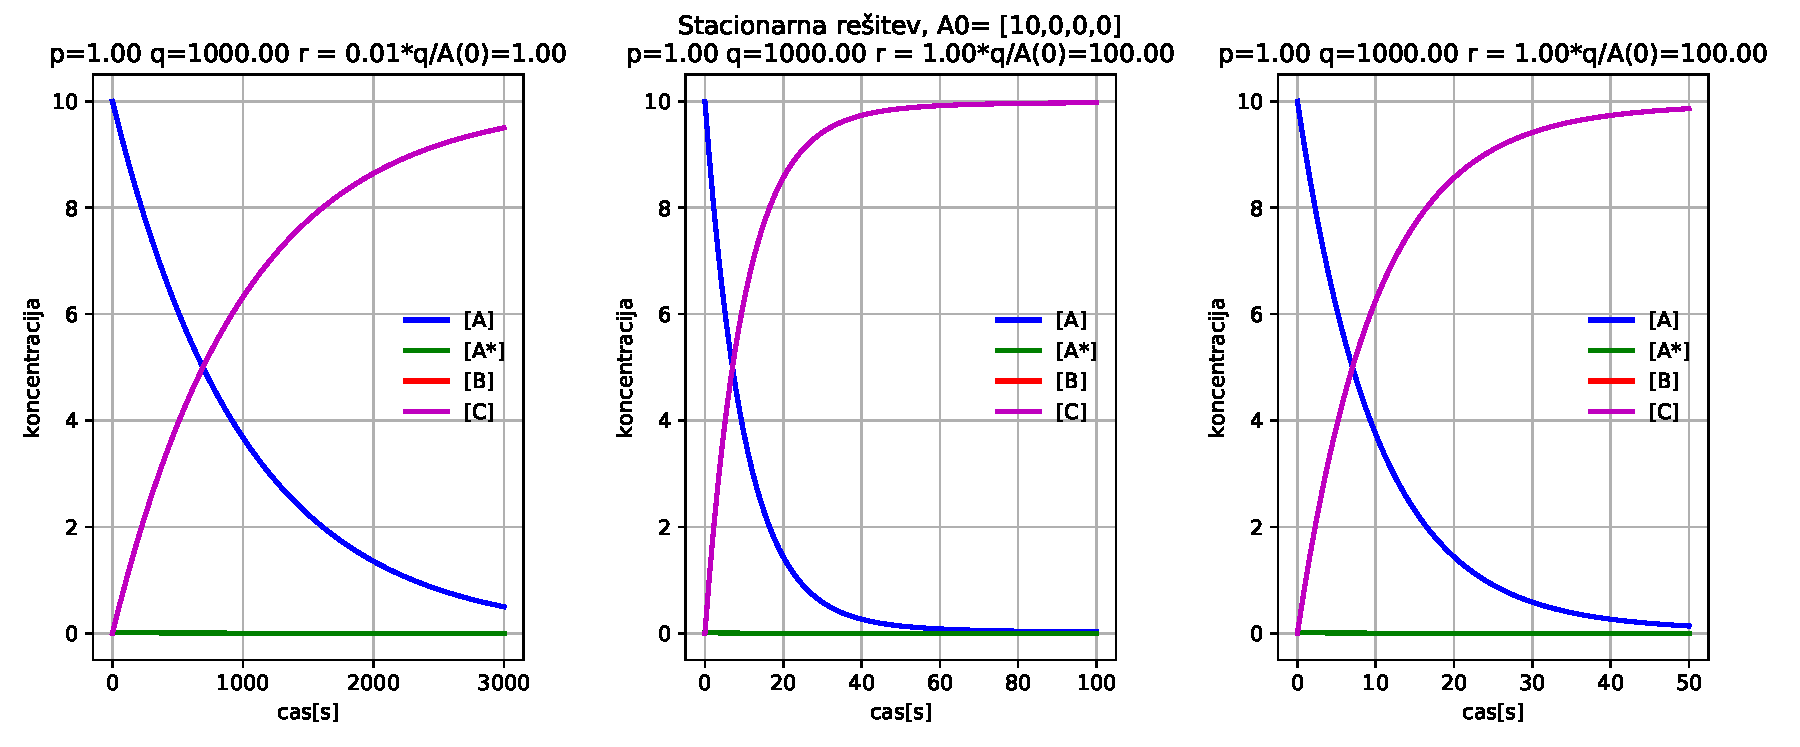
\includegraphics[width=20cm]{prva_stacionarna_resitev_skoraj_isto.pdf}
  \caption{Približek stacionarnega stanja nam da skoraj enako rešitev.} 
\end{figure}


\section{Vodikov bromid}
Poglejmo si sedaj primer reakcije nastajanja vodikovega bromida
\begin{equation}
 \ce{H_2 + Br_2 <=>2HBr}
\end{equation}
Ta je sestavljena iz vmesnih faz
\[
 \ce{Br_2 <=>[\ce{p}][\ce{q}] 2Br}
\]
\[
 \ce{Br + H_2 <=>[\ce{r}][\ce{s}]HBr + H}
\]
\[
 \ce{H + Br_2 ->[\ce{t}]HBr + Br}
\]

Očitno je, da sta tako Br in H prehodna reagenta, ki podobno kot A* v prejšni reakciji dosežeta stacionarno stanje, torej kar nastane tudi gre. \textbf{Pri H je to očitno, saj ves H, ki nastane reagira na koncu z $Br_2$ le v eno smer. Za $Br$ pa to pomeni, $p,q$ pa to pomeni $p>q$ in prav tako $r>s$. To pomeni da gledamo primer, ko je reakcija usmerjena v nastajanje HBr.}\newline\newline
Zapišimo logistični model za set reakcij (8).
\[
\dot{[H_2]} = -r[H_2][Br]+s[HBr][H],
\]
\[
\dot{[Br_2]} =  -p[Br_2]+q[Br]^2-t[H][Br_2],
\]
\begin{equation}
\dot{[HBr]} = r[Br][H_2]-s[HBr][H]+t[H][Br_2],
\end{equation}
\[
\dot{[H]}=0=r[Br][H_2]-s[HBr][H]-t[H][Br_2],
\]
\[
\dot{[Br]}=0=2p[Br_2]-2q[Br]^2-r[H_2][Br]+s[HBr][H]+t[H][Br_2].
\]
Sedaj izrazimo vrednosti H in Br ter vstavimo v ostale enačbe pa dobimo sistem:
\begin{equation}
\dot{[H_2]}= \dot{[Br_2]}=- \frac{1}{2}\frac{k[H_2][Br_2]^{1/2}}{\frac{[HBr]}{[Br_2]}+m}
\end{equation}
in
\begin{equation}
\dot{[HBr]} =  \frac{k[H_2][Br_2]^{1/2}}{\frac{[HBr]}{[Br_2]}+m},
\end{equation}
kjer sta $k$ in $m$
\begin{equation}
k = 2r\sqrt{\frac{p}{q}}\frac{t}{s}; \quad m=\frac{t}{s}.
\end{equation}
torej vidimo, da empirični model, ki ga predpostavljajo kemiki temelji na stacionarnem stanju vodikovega in bromovega iona. Konstanta m vpliva na hitrost nastajanja HBr v primerjavi z izgubo, $k$ pa prav tako določa usmeritev reakcije. \newline\newline
\begin{figure}[H]
\hspace*{-2cm}     
  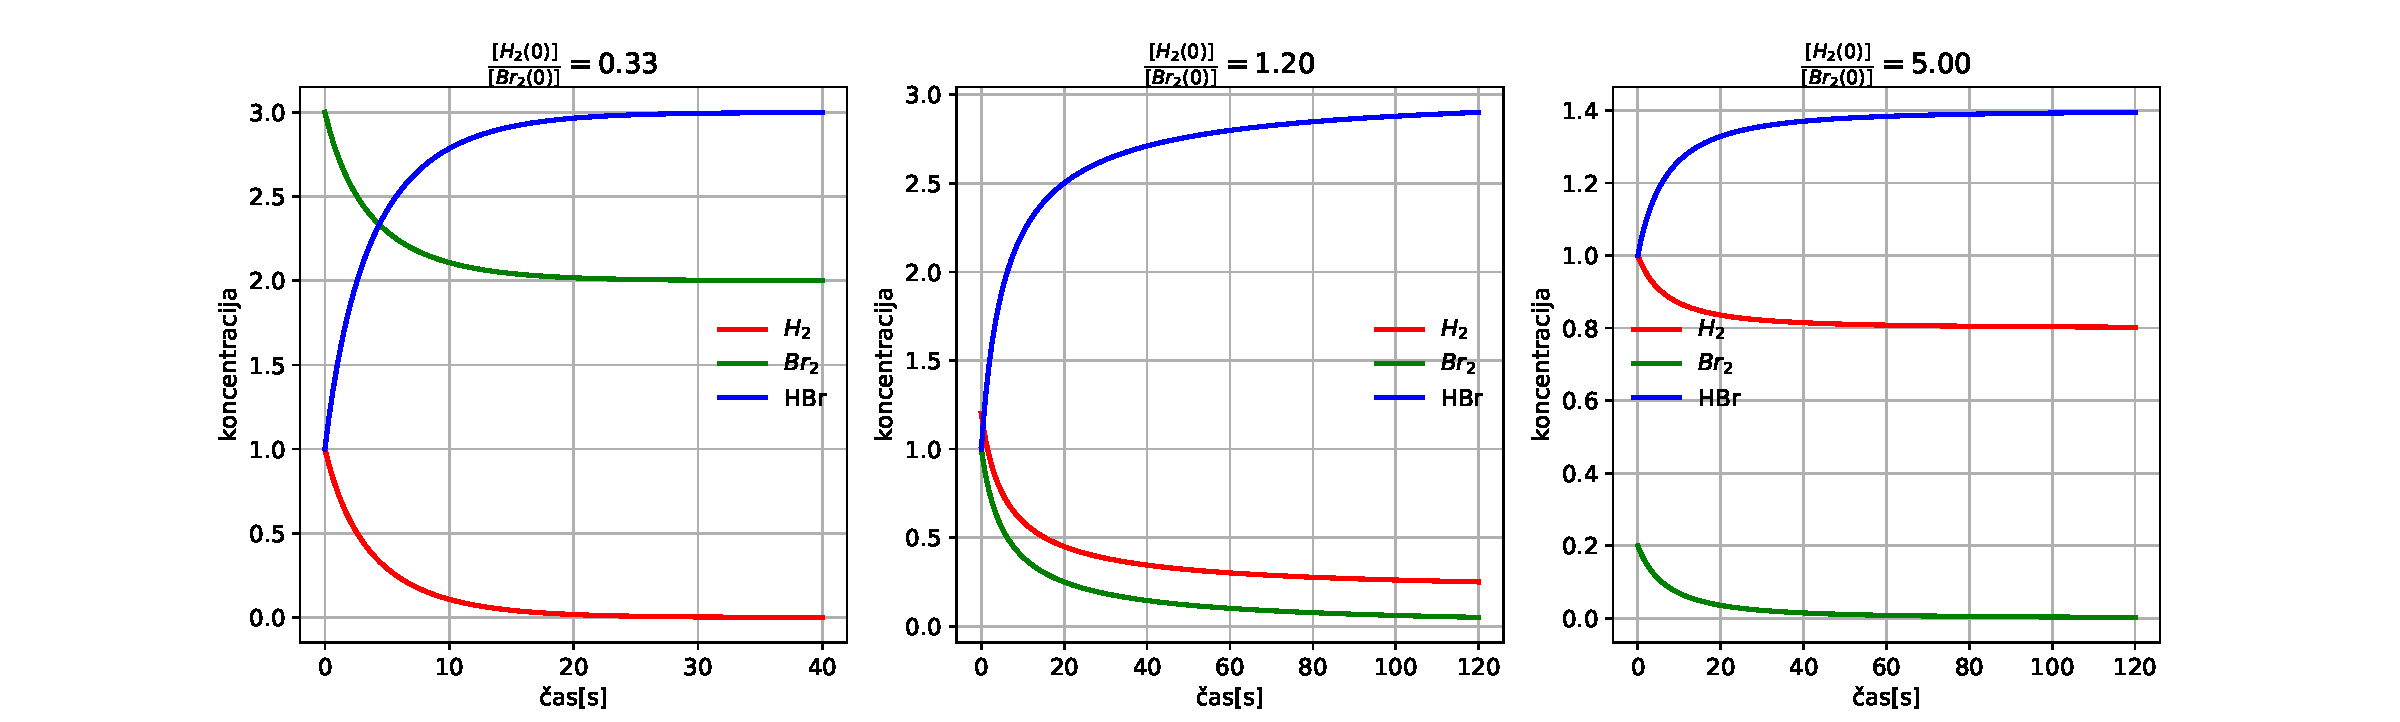
\includegraphics[width=20cm]{bromid_hitrost_relaksacije.pdf}
  \caption{Različne začetne koncentracije vodika in broma vplivata na čas relaksacije reakcije. Vidimo tudi, da se vodik in brom enako obnašata v času, ker je njuno spreminjanje enako } 
\end{figure}
\begin{figure}[H]
\hspace*{-2cm}     
  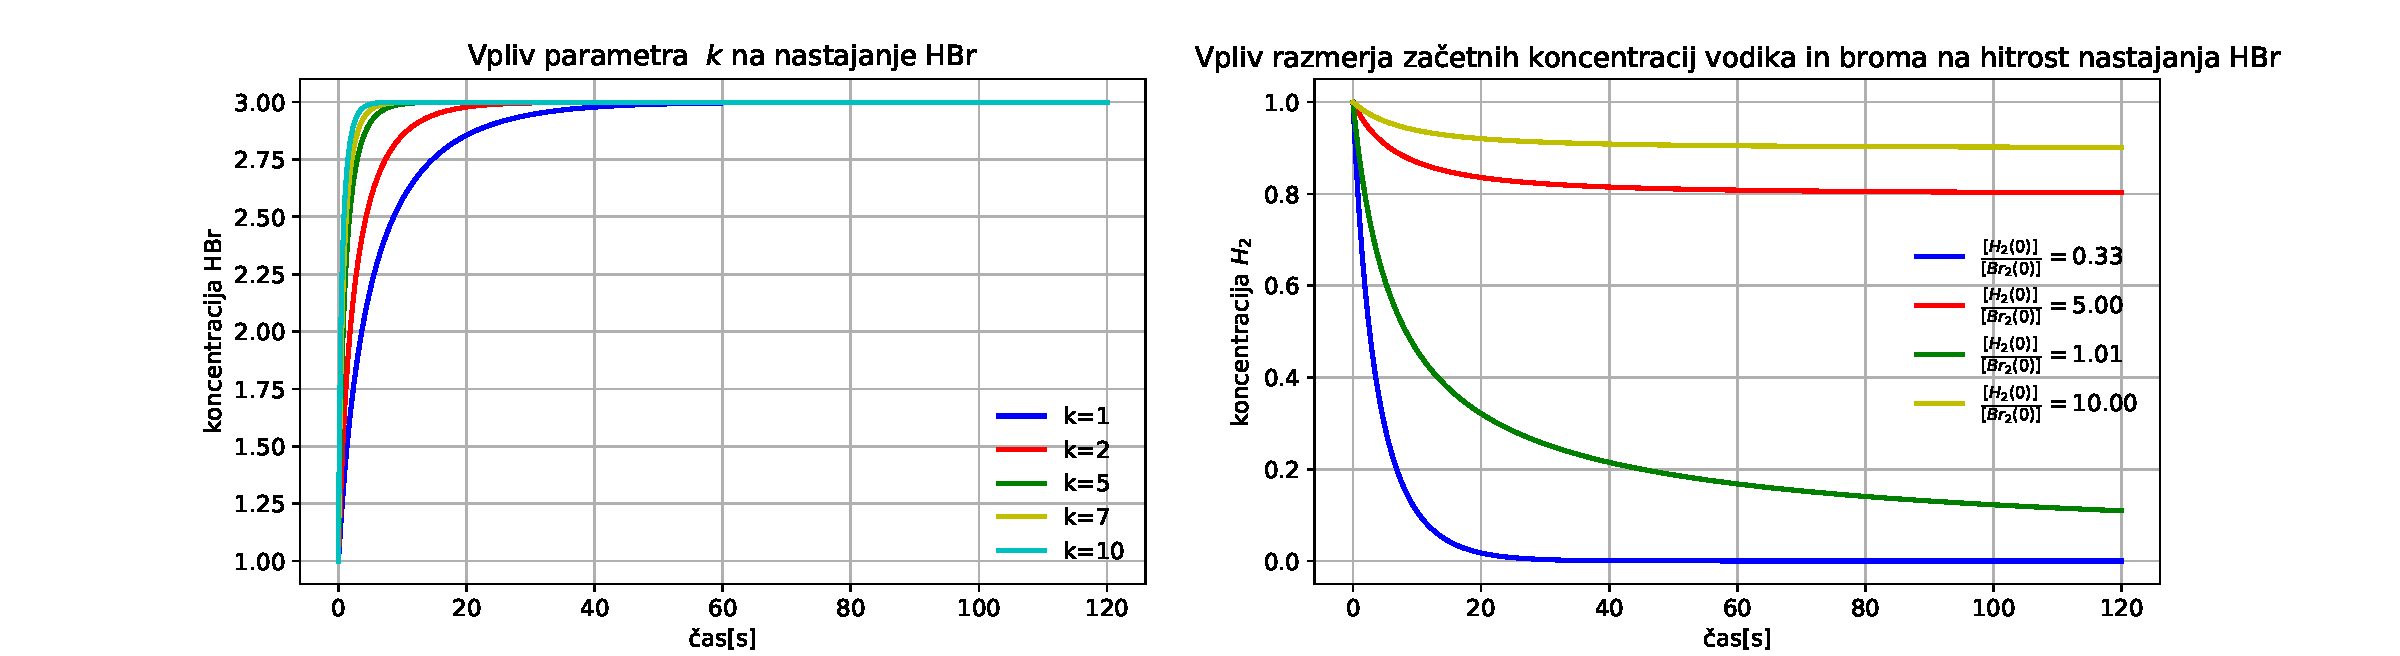
\includegraphics[width=20cm]{vodikov_vpliv_k.pdf}
  \caption{Levo: Parameter $k$ nam poveča hitrost reakcije v smeri nastajanja HBr, kar je očitno iz definicije. Desno: hitrost upada vodika je odvisna od začetne koncentracije vodika in broma. Vidimo, da do reakcije v primeru, ko je premalo broma na začetku sploh ne bo prišlo (rumena črta). Najbolj ugodno je zagotovo razmerje $50:50$. } 
\end{figure}


\section{Jodova ura}
V kemiji so leta 1886 odkrili reakcijo s katero so lahko v živo opazovali kemijsko kinetiko. Če recimo iodidne ione, ki so brezbarvni primešamo k persulfatu $IS_2O_8^{3-}$, se bo ta počasi spreminjal v jod, ki pa je vijolične barve, vendar pa dokler imamo na voljo tiosulfat $S_2O_3^{2-}$, ta \textbf{zelo hitro} reagira s jodom in tako vrne nazaj jod v stanje iodidnih ionov, ki so prosojni; \textbf{Dokler imamo na voljo tiosulfat v naši reakciji ne bo joda, ko pa ga bo zmanjkalo pa zelo hitro ne bo več zmanjševanja joda oziroma se bo tako spojina obarvala}. Na tak način bi lahko zelo nenatančno umerili čas sekunde, ki bi bil odivsen od začetnih koncentracij reagentov.
\begin{equation}
\textbf{\ce{IS_2O_8^{3-} + I^{-} ->[\ce{q_1}] I_2 + 2SO_4^{2-}}}
\end{equation}
\begin{equation}
 \textbf{\ce{IS_2O_3^{-} + I_2 ->[\ce{q_2}] I^- + S_4O_6^{2-}}}, 
\end{equation}
Vemo da je verjetnost za drugo reakcijo veliko večja od prve $q_1 << q_2$. \newline\newline
Reakciji imata tudi vmesno stopnjo, ki jo lahko opišemo, kot prehodno stanje, kjer so hitrosti reakcije za vmesno stanje veliko manjše kot hitrosti iz vmesnega v končno stanje. Podobno, kot v zgornjih primerih to pomeni, da se koncentracija vmesnih stanj skoraj ne spreminja, saj vse kar nastane takoj tudi reagira, in je tako upravičen približek stacionarnega stanja za $IS_2O_8^{3-}$ in $IS_2O_3^{-}$.
\[
\ce{S_2O_8^{2-} + I^{-} ->[\ce{p_1}] IS_2O_8^{3-}},
\]
\[
\ce{IS_2O_8^{3-} + I^{-} ->[\ce{q_1}] I_2 + 2SO_4^{2-}};
\]

\[
\ce{S_2O_3^{2-} + I_2 ->[\ce{p_2}] IS_2O_3^{-} + I^-},
\]
\[
\ce{IS_2O_3^{-} + S_2O_3^{2-} ->[\ce{q_2}] I^- + S_4O_6^{2-}},
\]
Tako dobimo
 $[IS_2O_8^{3-}]=\frac{p_1}{q_1}[S_2O_8^{2-}]$ in $[IS_2O_3^{-}]=\frac{p_2}{q_2}[I_2]$, ,ki jih vstavimo v enačbe zgoraj, ter tako dobimo
\begin{equation}
\dot{[I^-]} = -2p_1[I^-][S_2O_8^{2-}] + 2p_2[S_2O_3^{2-}][I_2],
\end{equation}  
\begin{equation}
\dot{[I_2]} = p_1[I^-][S_2O_8^{2-}] -p_2[S_2O_3^{2-}][I_2],
\end{equation}  
\begin{equation}
\dot{[S_2O_3^{2-}]} = -2p_2[I_2][S_2O_3^{2-}].
\end{equation}
Vidimo, da parametra $q_1$ in $q_2$ v približku stacionarnega stanja ne vplivata direktno na potek reakcije, ampak le na vrednosti vmesnih produktov. Tako je torej reakcija določena s parametroma $p_1$ in $p_2$, ki so lahko v različnih razmerjih. Persulfata je v sistemu mnogo več kot ostalih zato privzamemo, da je njegova koncentracija konstantna. \newline\newline
Definirajmo
\[
\frac{p_2}{p_1} = \lambda.
\]
\begin{figure}[H]
\hspace*{-2cm}     
  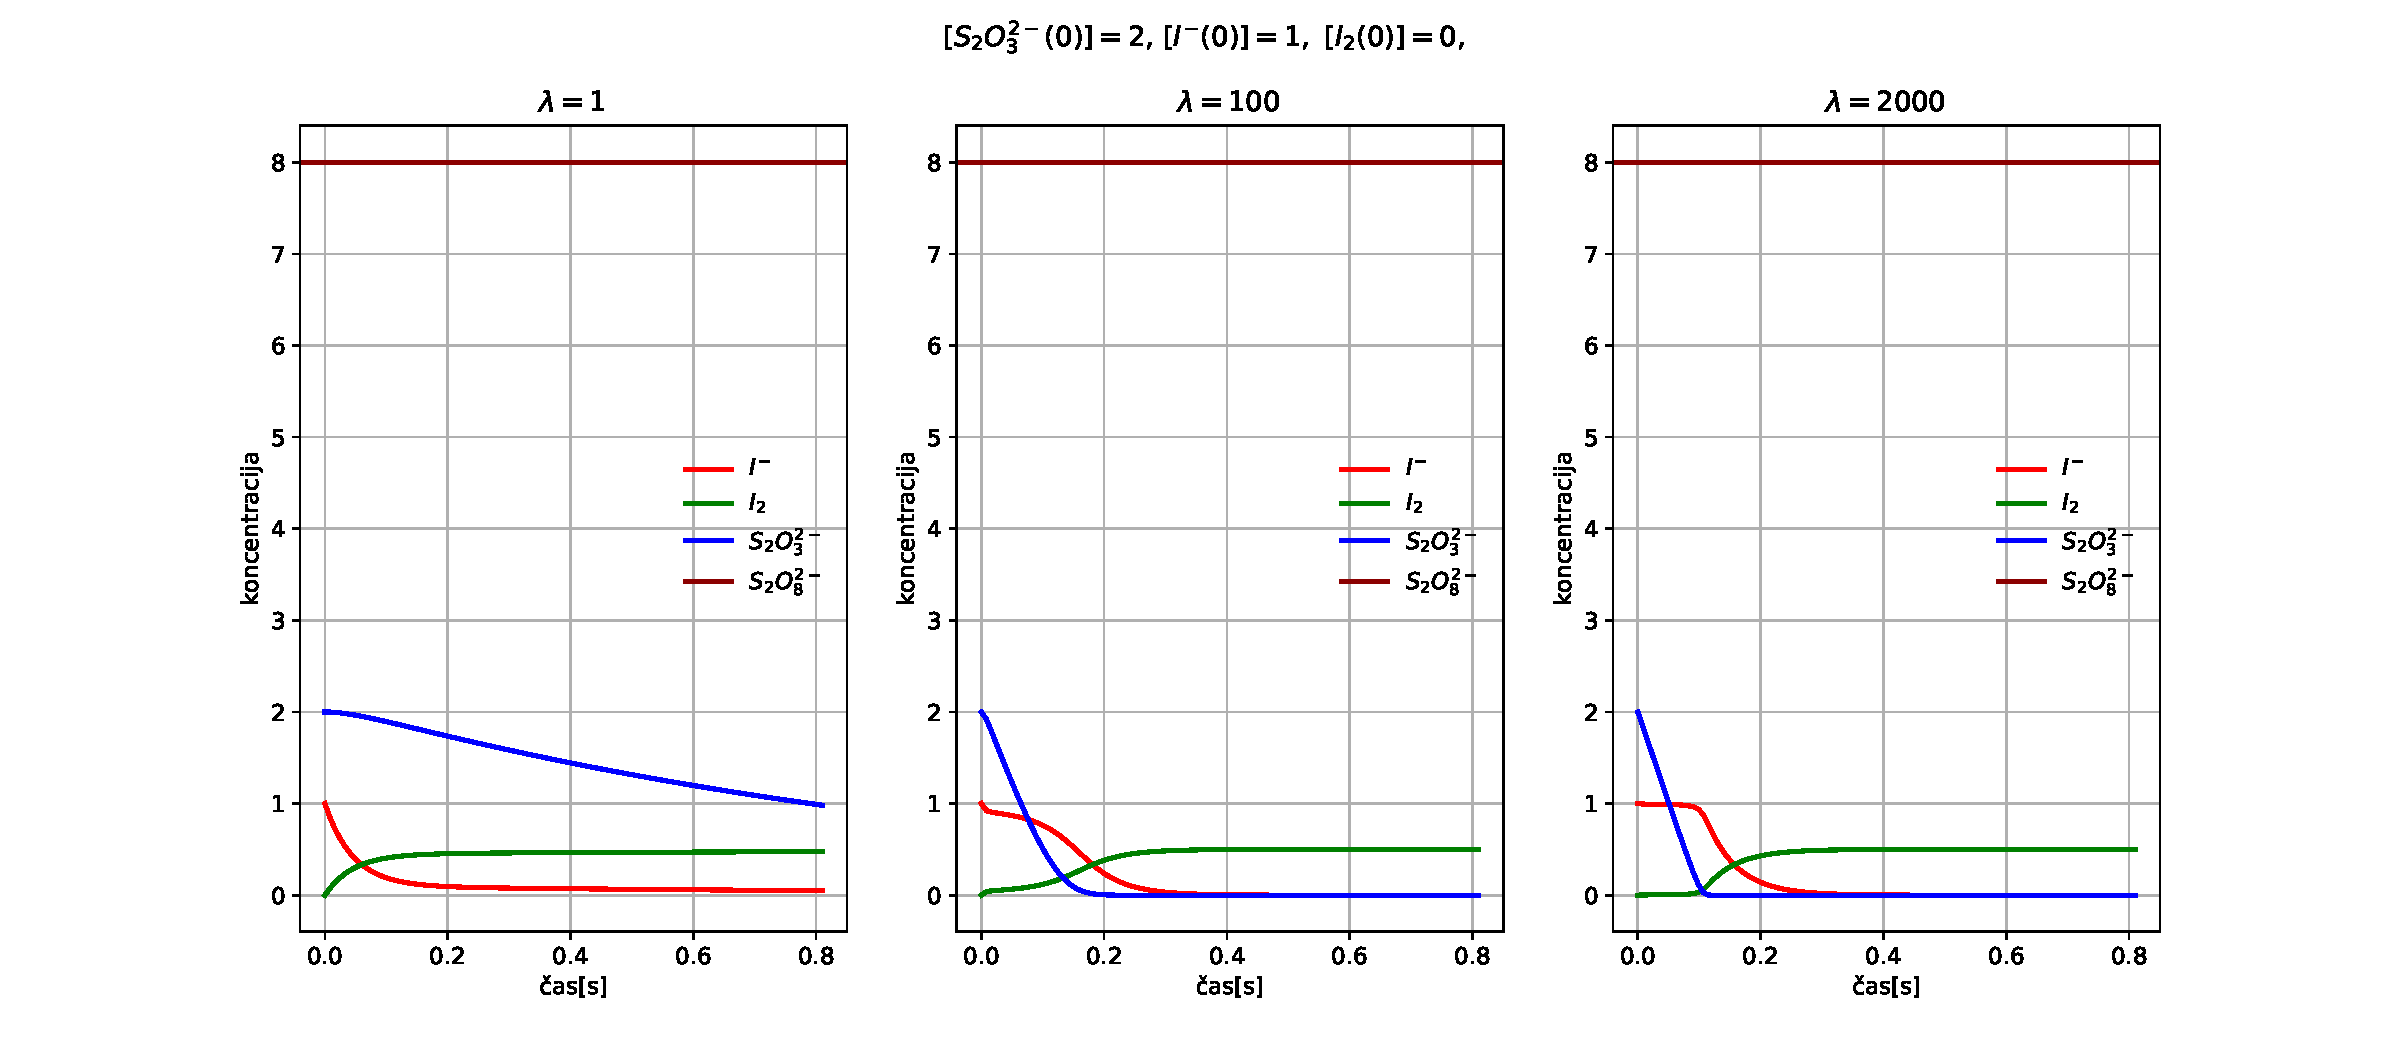
\includegraphics[width=20cm]{jodova_ura_1.pdf}
  \caption{Vpliv razmerja hitrosti reakcij na jodovo uro. Vidimo da mora biti za nastanek ostrega prehoda velik lambda oziroma hitrost izginjanja joda veliko večja hot hitrost nastajanja joda, dokler imamo tiosulfat v sistemu. Tak pogoj je očitno izpoljnen za reakcijo jodove ure. } 
\end{figure}
\begin{figure}[H]
\hspace*{-2cm}     
  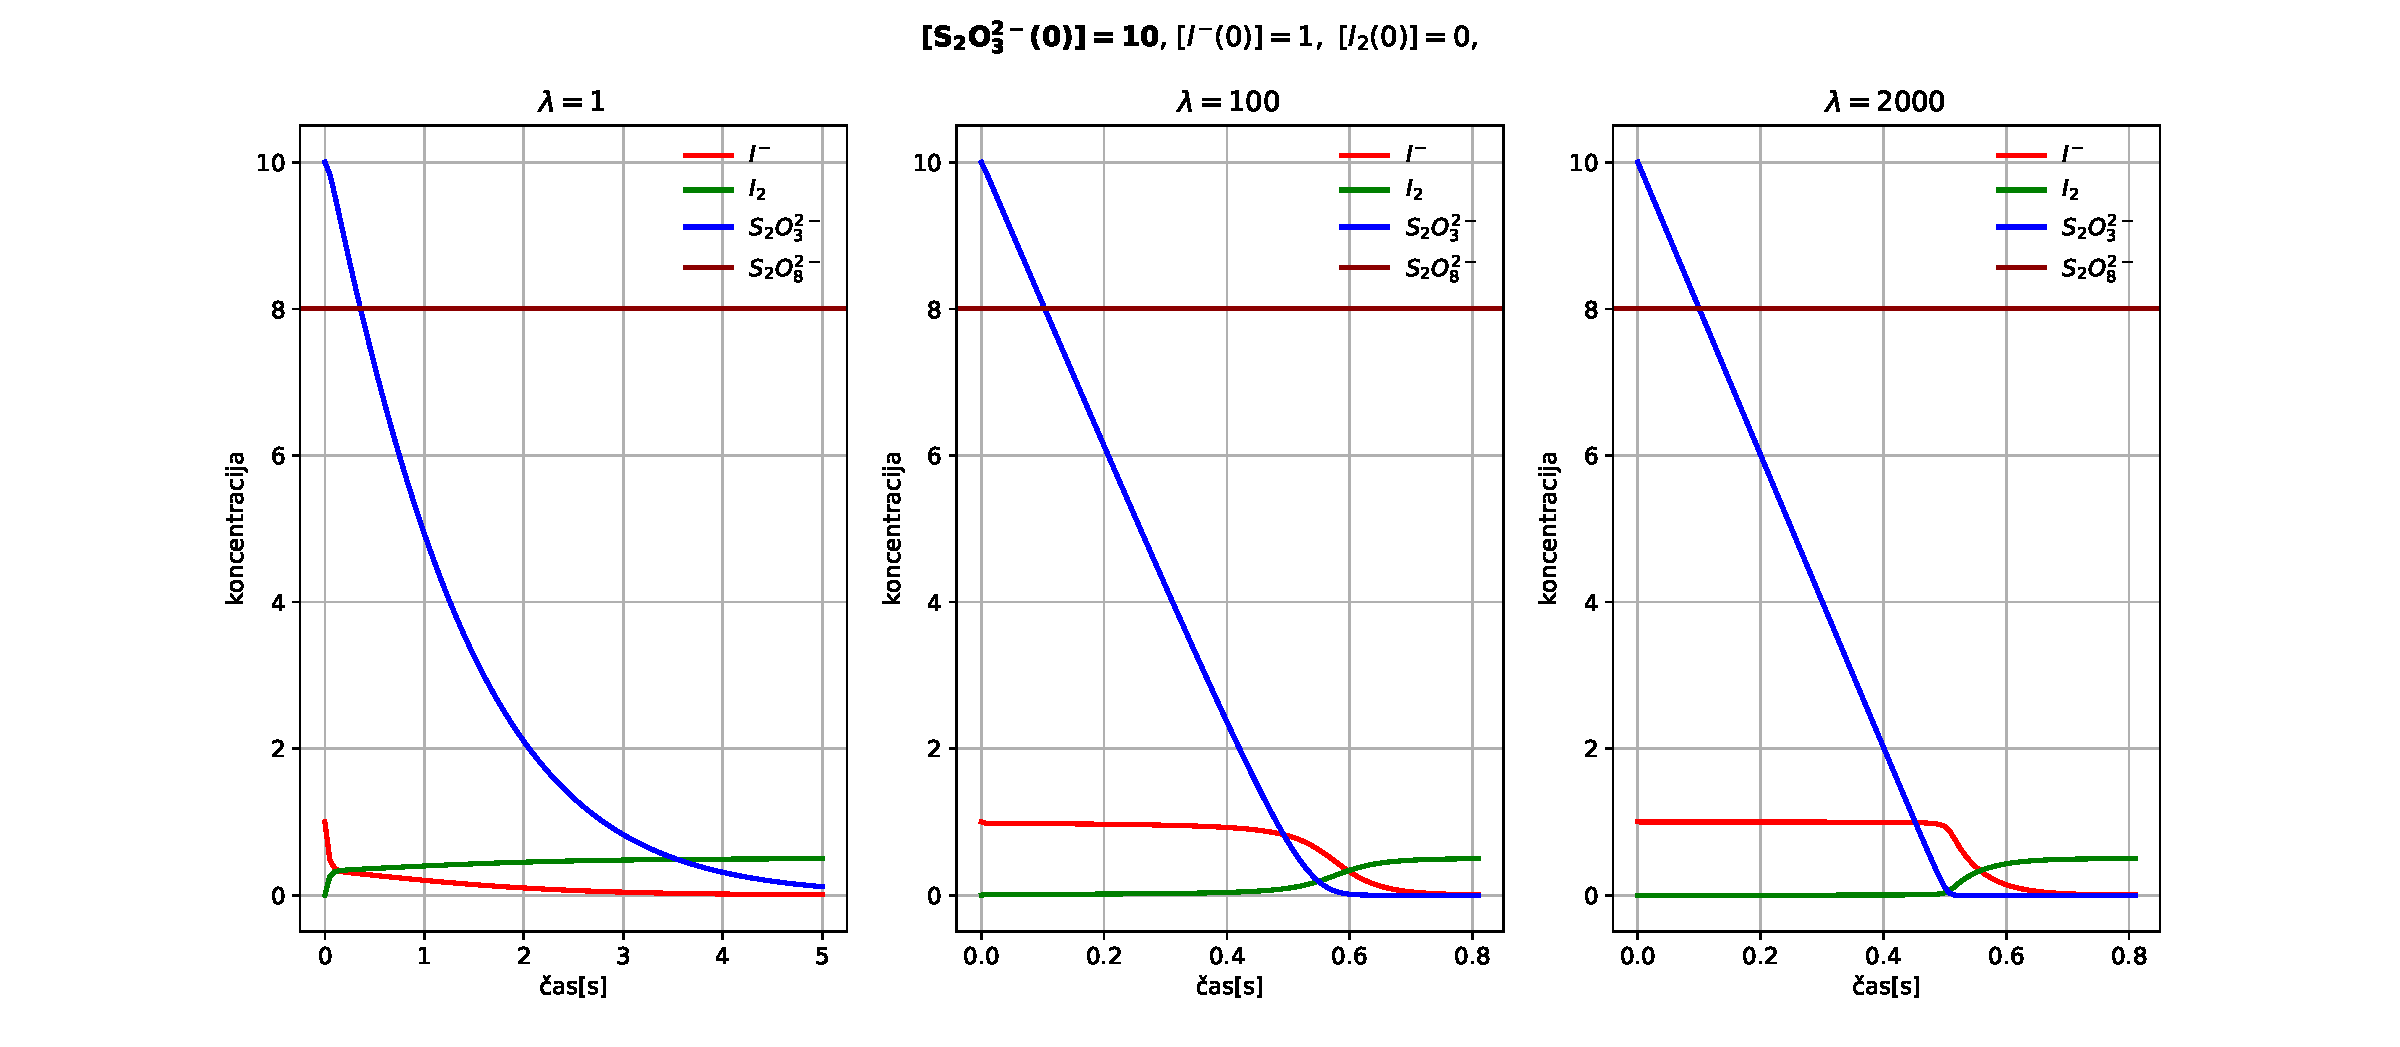
\includegraphics[width=20cm]{jodova_ura_2_daljsanje_casa.pdf}
  \caption{Čas začetka nastajanja joda (karakterističnega časa ure) je povezan s začetno koncentracijo tiosulfata, saj ta omogoča razpad joda nazaj v jodidne ione. Na strmino razmaha ure pa koncentracija tiosulfata ne vpliva.} 
\end{figure}
\begin{figure}[H]
\hspace*{-2cm}     
  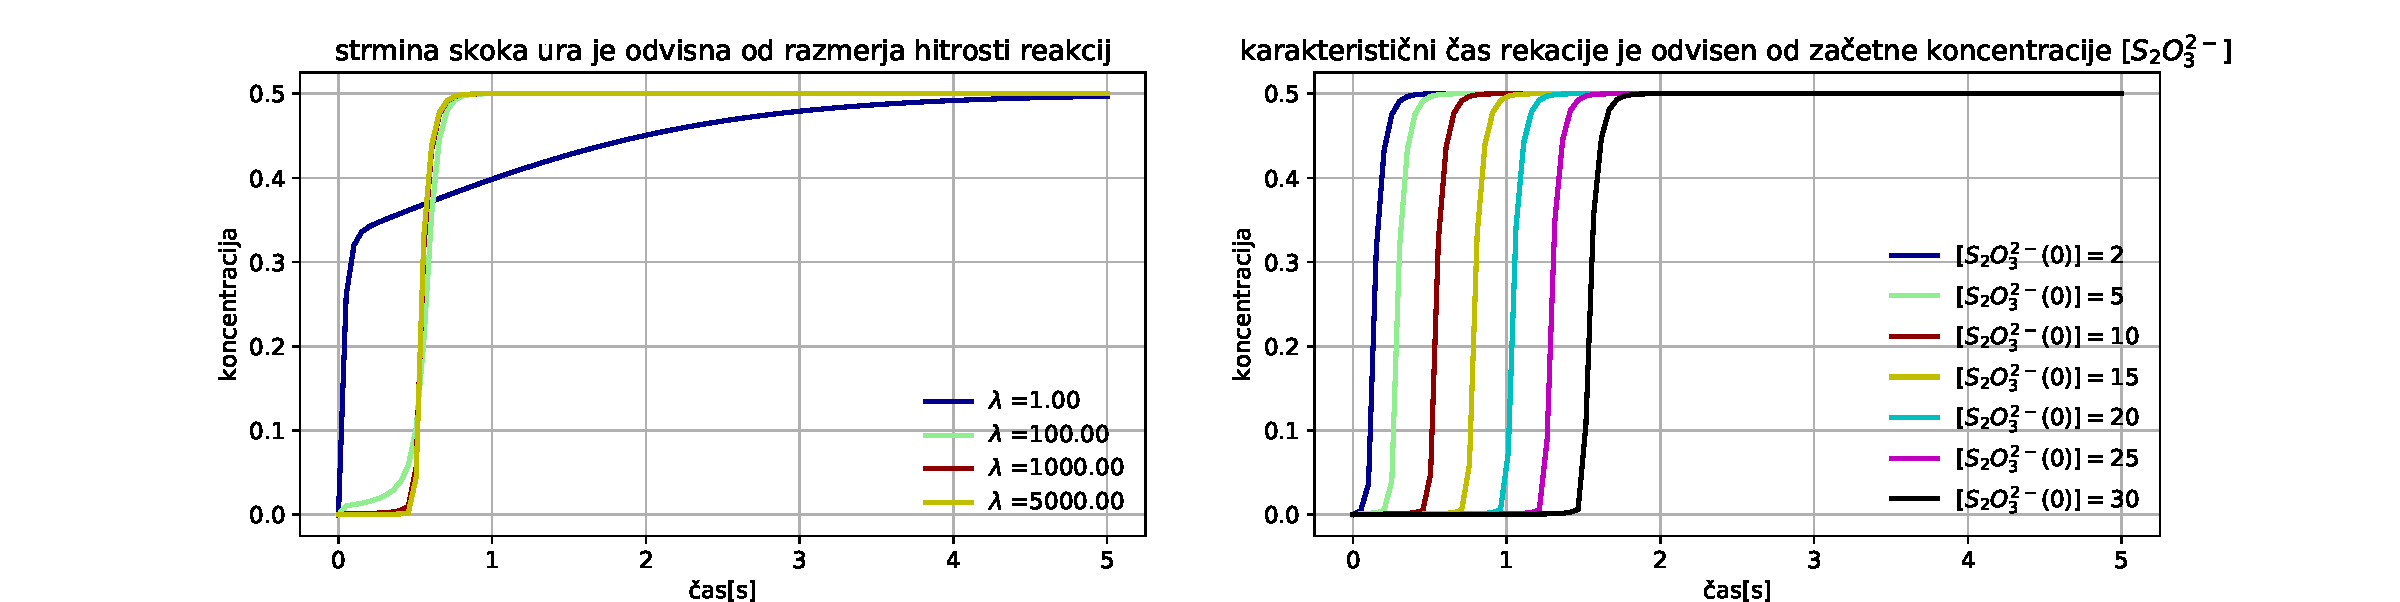
\includegraphics[width=20cm]{jodova_ura_2_karakteristika.pdf}
  \caption{Levo : vpliv lambda na strmino prehoda na levi in vpliv tiosulfata na čas razmaha joda na desni.} 
\end{figure}
Seveda na karakteristiko ure vpliva tudi začetna koncentracija jodidnih ionov, na sliki (10) spodaj, saj je tako večja možnost nastanka joda, ki porabi tiosulfat, zato je čas ure krajši.

\begin{figure}[H]
\hspace*{-2cm}     
  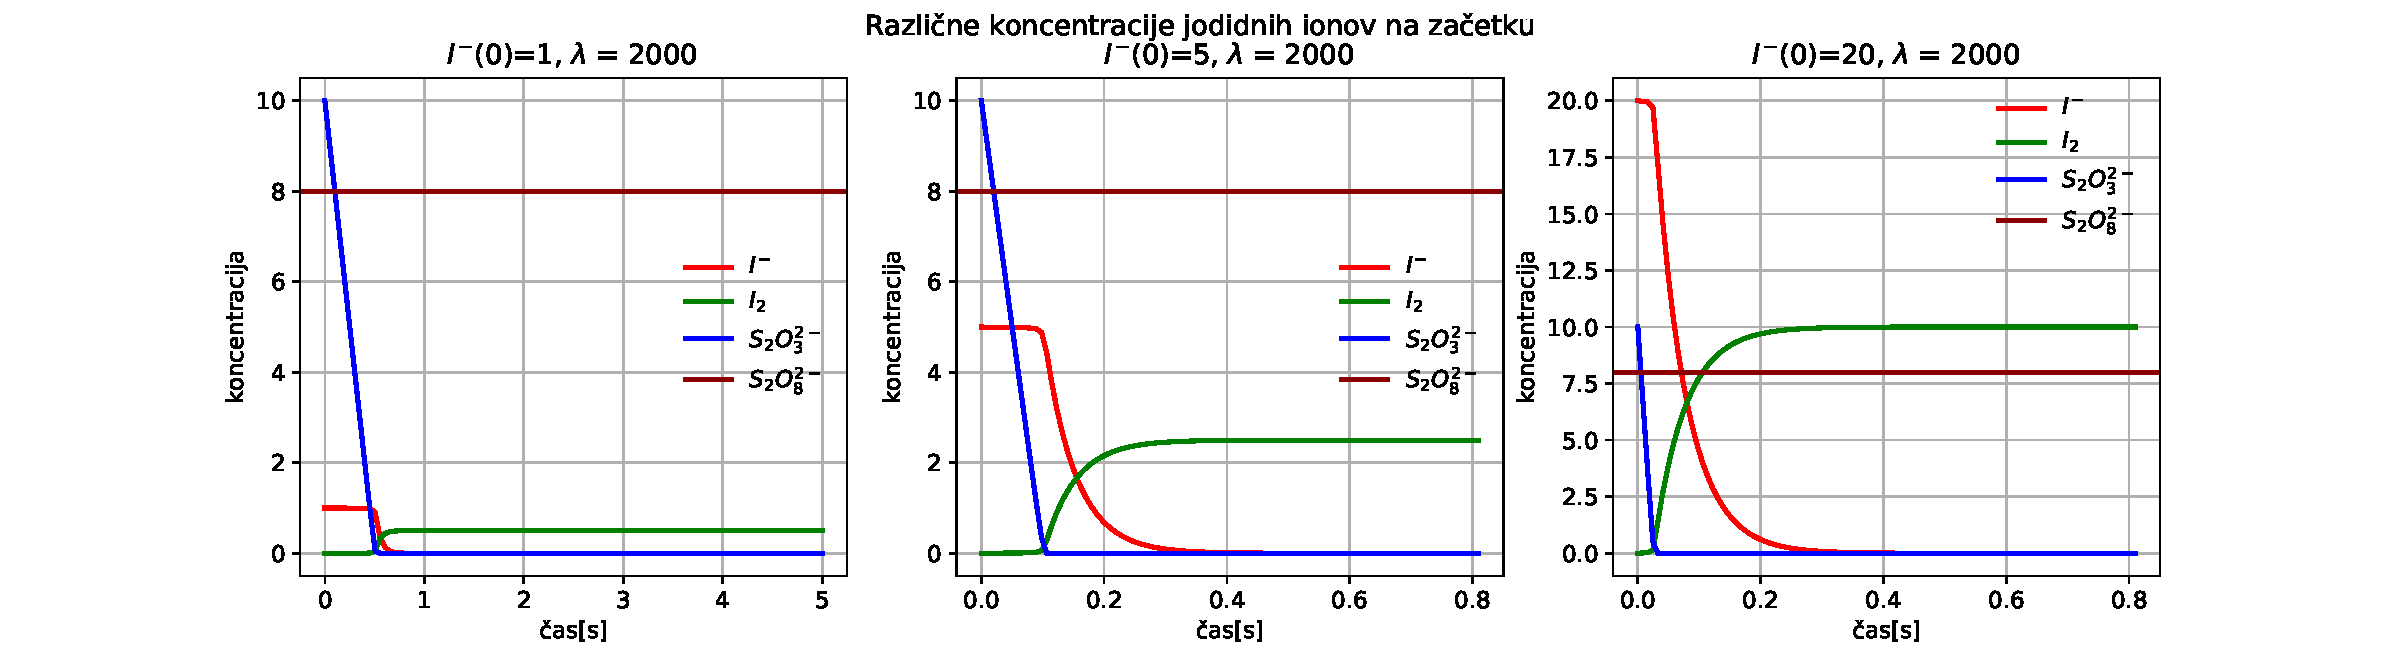
\includegraphics[width=20cm]{jodova_ura_2a_daljsanje_casa_jod.pdf}
  \caption{Vpliv iodidnih ionov je neposreden in posreden. Neposredno bo zaradi več iodidnih ionov na začetku ob reakciji s persulfatom nastalo več končnega joda. Posredno pa bo večja koncentracija jodidnih ionov na začetku vplivala na hitrost porabljanja tiosulfata in stem zmanjšala karakteristični čas ure.} 
\end{figure}
\section{Zaključek}
S populacijskimi modeli se da lepo opisovati tudi kemijske reakcije, kar je sigurno uporabno za preučevanje hitrosti za različne reakcije in kinetiko kemijskih reakcij. Čas ure je odvisen od razmerja hitrosti reakcij in začetnih vrednosti reaktantov. Obstajajo tudi kemijske reakcije, ki so periodične, torej je hitrost spreminjanja enega odvisna od drugega in obratno, da dobimo harmonični sistem. To so lahko prave ure, ki pa seveda ne bodo tako natančne, kot so mehanske ali atomske ure.

%\lambda=\frac{\widetilde{q}}{\widetilde{p}}=
\end{document}